\section{Bewertung}
\label{sec:abschn3}
Wir haben erfahren, dass Strassens Algorithmus in $\Theta(n^{lg\;7})$ läuft, wobei n für
die Anzahl der Zeilen eine Matrix steht. Somit soll der Algorithmus in der Praxis schneller als die zwei anderen Algorithmen laufen. Mit einer Implementierung in der Programmiersprache Java werden die drei Algorithmen auf verschiedene Matrixgrößen angewendet und getestet. Die Matrizen werden zufällig generiert und in den jeweiligen Algorithmus eingegeben. 

In Abbildung \ref{1} ist die Laufzeit in benötigten Zeiteinheiten pro Matrixgröße abgebildet. Eine Unstimmigkeit wird direkt festgestellt; Strassens Algorithmus ist langsamer als das \enquote{naive} Verfahren. Die Ursache liegt in der rekursiven Implementierung. In einer ersten Variante wird der Basisfall auf $n = 1$ gesetzt und somit werden die Matrizen soweit aufgeteilt, bis der Basisfall erreicht wird. Dadurch entsteht ein Rekursionsstack mit hoher Größe, deren Verwaltung viele Ressourcen verbraucht.

\begin{figure}[H]
    \center
    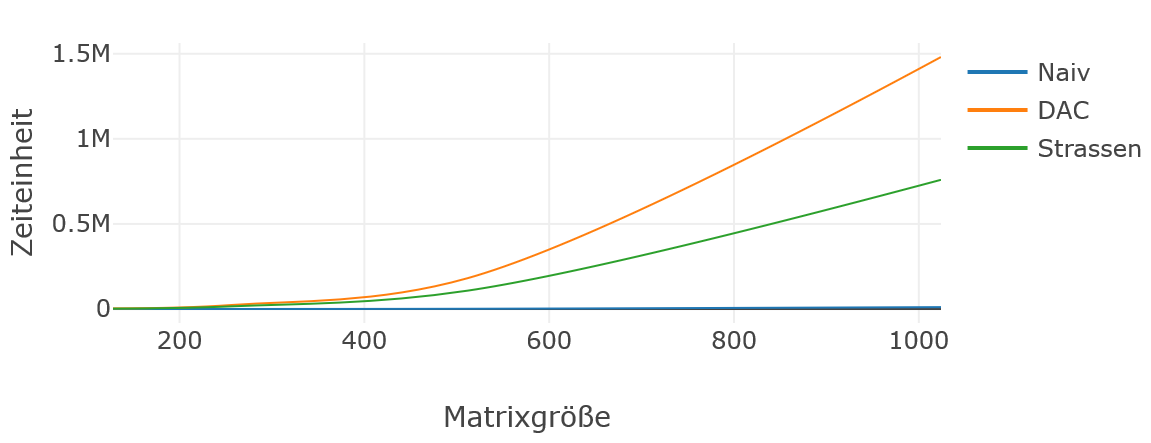
\includegraphics[scale=0.38]{basisfallnot.png}
    \caption{Basisfall $n = 1$}
    \label{1}
\end{figure}

Beim Setzen des Basisfalls auf $n = 32$ ist eine klare Verbesserung in Abbildung \ref{32} zu sehen. Auf diese Weise werden die Matrizen $A$ und $B$ ab einer bestimmten Größe ($n = 32$) mit dem \enquote{naiven} Verfahren multipliziert, sodass die Matrizen nicht in viele kleinen Teilmatrizen aufgeteilt werden. Daher ist für die praktische Anwendung von Strassens Algorithmus einen geeigneten \enquote{Crossover}-Punkt für den Basisfall zu wählen.
\begin{figure}[H]
    \center
    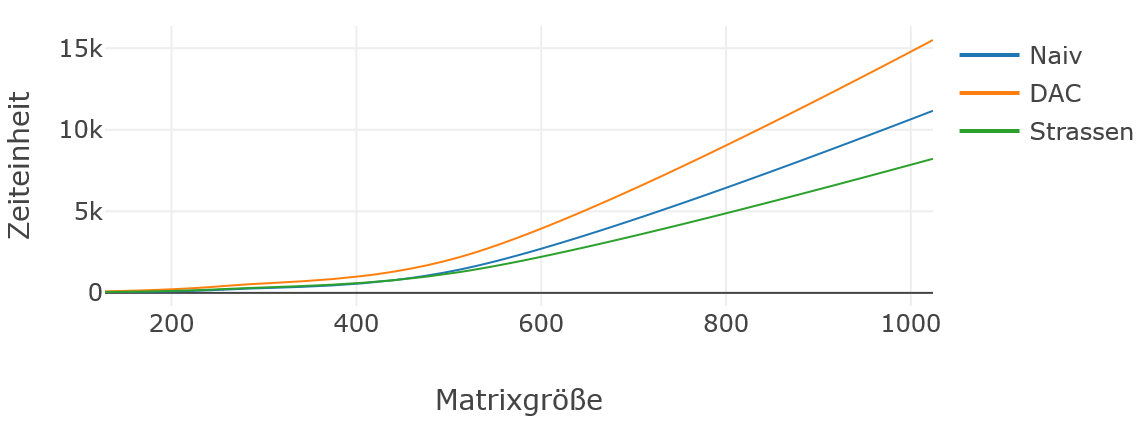
\includegraphics[scale=0.38]{basisfallmod.png}
    \caption{Basisfall $n = 32$}
    \label{32}
\end{figure}